\subsubsection{Overview}

The SmartRobotinoInstructionPlanner component is currently responsible of the task coordinantion between all components of the Robocup Logistics Software. The intention of the previous team was that a master robot should process the information from the Robocup Logistics Refereebox and start instruction all other robots. The scenario application like driving, docking or detection should be implemented in the SmartLispServer component using the SmartTCL language. \\

The SmartRobotinoInstructionPlanner is connected to the Refbox Component using a bi-directional SmartSoft port. For transmitting data between those two components various communication objects are used. To the other components like the SmartMPSDetection, SmartAlvarTagDetection or the components which provide services like mapping or driving, the SmartRobotinoInstructionPlanner uses SmartTCL messages which are transferred by using strings and communication ports. 


\subsubsection{Previous implementation}

As described in (reference to book of knowledge) the InstructionPlanner was designed for planning and coordination of other components on the master robotino (the one who manages the connection between the Refbox and all robotinos) but also all other robotinos. This means that it was designed that on all slave robotinos only the necessary parts like driving, detection or docking should run. All coordination should be done by the instruction planner on the master robotino. The intention behind this idea was that the referee box was sending a list of probable zone which can contain a MPS station for detection. This list of MPS stations was then splitted by an algorithm into three parts (one for each robot), so that a concurrent exploration and detection of the gamefield can be archieved. In the 2017 scenario (link to 2017 rules) this feature was discarded from the competition. In the newer scenario there is no information whether there is a MPS station or not. Therefore this feature was also discared in the new design for the 2017 competition \ref{sec:new_design}.  \\



\subsubsection{New Design}
\label{sec:new_design}
Describe the overall design of the instruction planner. Which ports are used and connected to other components. What are the tasks of the component and what purpose do they fulfill. 

\begin{figure}[h]
\centering
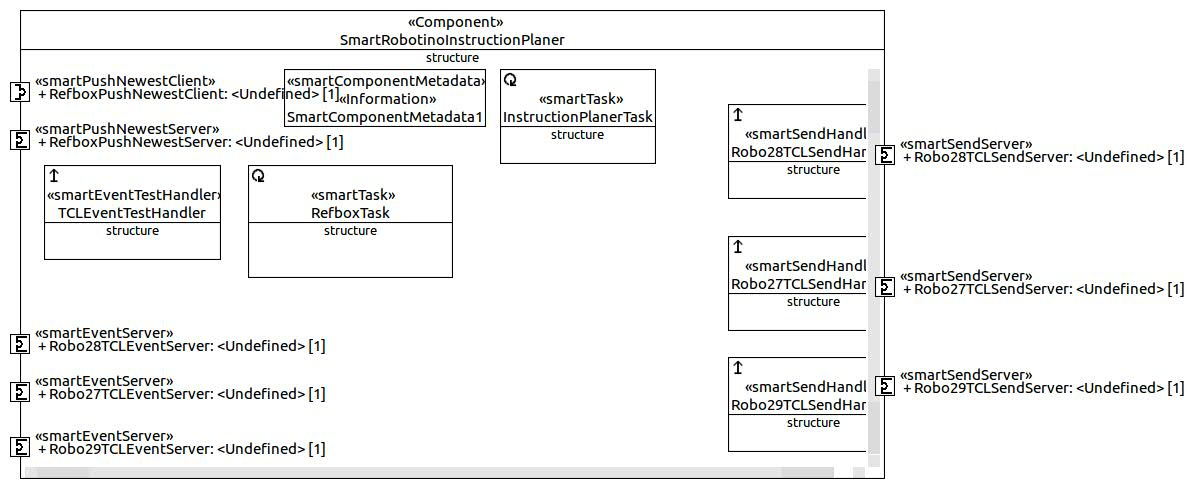
\includegraphics[scale=0.25]{pic/SmartRobotinoInstructionPlaner.JPG}
\caption{Model of InstructionPlanner}
\label{fig:i_overview}
\end{figure}


As shown in figure \ref{fig:i_overview} the SmartRobotinoInstructionPlanner has multiple input and output ports which are connected to components such as RefboxServer, MPSDetection or AlvarDetection. This connection is created over the SmartLispServer component using SmartTCL messages. On the other hand connections to the SmartLogisticsRefboxServer are done over communication objects which can be created inside smartsoft for data like the Phases, Maintenance and so on. For the connection between the Instruction Planner and the Refbox component a communication called CommRefbox is used. This object can be used to send certain data about the detected stations, exploration or production phase and the state of the robotino as seen by the 
Refereebox. \\

\newpage

Currently the CommRefbox communication object can be used to transmit the following data: 

\begin{itemize}

\item MessageType

This describes the message type. This needs to be done because in C++ the type of an object (even if we have polymorphism) can be not be derived. Therefore each message needs a message type. Valid message types are: GAMESTATE, EXPLORATION\_INFO, MACHINE\_INFO, MACHINE\_REPORT, ORDER\_INFO and 
ROBOT\_INFO. 

\item Gamestate

The gamestate part of the communication object can be used to transmit the current gamestate from the RefBoxServer to the InstructionPlanner. The elements of this submessage is the state, phase and a timestamp. 

\item ExplorationInfo (deprecated)

This was originally intended to transmit a set of zones which can include a MPS station for the team with a high probability. But because of new rules in the 2017 scenario this was dismissed. Therefore this message part is currently out of use. The explorationInfo contains a array of probable zones. 


\item machineInfos

The machineInfos message contains a list of six machineInfo which can be used as database for already detected MPS stations. The list of machineInfo begins with mInfo1 and ends with mInfo6.

\item machineInfo

The machineInfo message describes the position of a detected MPSstation with the X-Coordinate the Y-Coordinate and the orientation of the MPS-Station. This is exactly the data the Refereebox expects for a sucessfull detection of the station.


\item machineReport


The machineReport describes general information about the detected MPS stations. The informations which can be transmitted are the name of the MPS station, the zone where the MPS is localized, and the detected light signal. The lightsignal is deprecated in the 2017 scenario. 

\item robotInfo and robotState

These two message containers are used to transmit the current state of the robot as seen from the refbox. The state of the robot can be ACTIVE if everything works normal, MAINTENANCE if the team asked for a maintenance break to fix some issue of the robot or DISQUALIFIED if the robot was put into maintenance the second time or violated some rule of the contest. This message is used for internal monitoring of the contest from the robot site. For example if the robot returns from reconnects to the Referee Box from a maintenance break it can detect whether it can start to drive into the field again.  


\item orderInfo

//todo 


\end{itemize}


\subsubsection{Statemachine}

Describe the state machine with a diagram with states
and transitions

\subsubsection{Maintenance Modes}

Describe how to team and the robot can react to failures and the system. How to set the robot into maintenance mode and how the robot can return to the game. 


\subsubsection{Outcome}

Multiple robots and Production phase







